\chapter{Simulation Study}\label{ch:simulation-study}


\section{ParallelQueue Package}\label{sec:parallelqueue-package}
%======================================================================
In order to generate and study parallel queueing processes, few trivial options currently exist.
Moreover, while there exist some discrete event simulation (DES) frameworks which indeed focus on queueing networks, they currently tend not to permit the simultaneous study of asynchronous, redundancy-based schemes~\cite{noauthor_ciwpythonciw_nodate}.
In order to visualize and analyse the large class of queueing systems within this paradigm~\cite{shneer_large-scale_2020,cruise_stability_2020}, I introduced a novel module for Python which is currently available on PyPi: \textit{ParallelQueue} extending the DES package \textit{SimPy}.

The package currently allows for the studying of parallel systems with or without redundancy as well as with the option of allowing thresholds to be implemented in either case.
Moreover, the package allows one to specify any inter-arrival and service time distribution as well as their own \lstinline{Monitor}s, being a class which can gather data from the ongoing simulation to be distributed back to the user upon the completion of a simulation.
In particular, the \lstinline{Monitor}s are currently configured to collect data upon arrival, routing, and job completion as demonstrated by Figure~\ref{fig:API}.

Take Figures~\ref{fig:red} and~\ref{fig:redpic} for example, which permits one to simulate a Redundancy-2 queueing system with 100 queues in parallel for 1000 units of time while returning the total queue counts over time (which are updated upon a change in queue count).

\begin{figure}

    \begin{lstlisting}[label={lst:lstlisting}]
#!/usr//bin/python3
from parallelqueue.base_models import RedundancyQueueSystem
from parallelqueue.monitors import TimeQueueSize
import random

sim = RedundancyQueueSystem(
                    maxTime=1000.0,parallelism=100, seed=1234,
                    d=2, Arrival=random.expovariate,
                    AArgs=9, Service=random.expovariate,
                    SArgs=0.08, Monitors = [TimeQueueSize])
# Note RedundancyQueueSystem is a ParallelQueueSystem wrapper
sim.RunSim()
totals = sim.MonitorOutput["TimeQueueSize"]
    \end{lstlisting}
    \caption{Python code using \textit{ParallelQueue} to simulate a Redundancy-2 System.}
    \label{fig:red}
\end{figure}

\begin{figure}
    \centering
    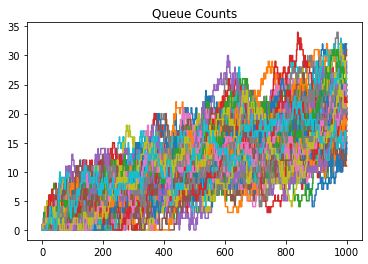
\includegraphics[scale=0.8]{redundancy}
    \caption{Plot using \lstinline{totals} of Figure~\ref{fig:red}}
    \label{fig:redpic}
\end{figure}

Remarkably, the simulation itself is performed speedily on consumer hardware despite the size of the system as demonstrated in Figure~\ref{fig:lstlisting2}.
\begin{figure}
    %! suppress = MissingLabel
    \begin{lstlisting}
CPU times: user 2.02 s, sys: 9.57 ms, total: 2.03 s
Wall time: 2.05 s
Intel i5-8250U (8) @ 3.400GHz
    \end{lstlisting}
    \centering
    \caption{Runtime Statistics}
    \label{fig:lstlisting2}
\end{figure}


Altogether, this makes the package easy to parallelize with and thus to compare systems of different sizes
and with large running-times.
While currently not implemented in any development branch of \textit{ParallelQueue}, the base Python package
\textit{multiprocessing} is used in throughout this paper when simulating for the same system across parameters.
In general, the main caveat when processing many models is that the storage of the simulation results can quickly begin
to consume storage;
when processing many models, therefore ensure that they are saved (e.g., using \textit{pickle}) and removed from
the local environment when doing analysis.

In terms of development, the models implemented in the \textit{base\_models} module use the framework established in~\ref{ch:model-specification}.
That is, modelling redundancy, a hyperedge of sorts is generated whence the dispatcher
receives a job to be cloned.
This hyperedge then exists for the duration of time for which the replica class is in the system and is defined in such
a way that \textit{Monitor} class objects can interact with them in order to acquire data.
In Python, such a data structure can be implemented rather easily by employing the \textit{Dict} type which defines
a keyed set of values.
By keying based on the job arrivals (before cloning), a unique set of marks can be retrieved for the set by simply using
the \textit{Dict} object as a reference.

\begin{figure}
    \centering
    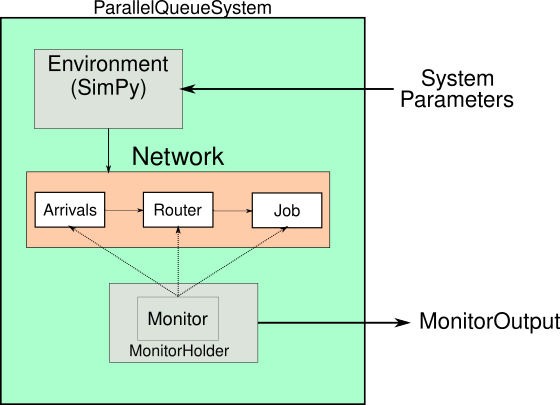
\includegraphics[scale=0.7]{pq}
    \caption{Overview of the ParallelQueue API}
    \label{fig:API}
\end{figure}


\section{Results}\label{sec:results}
First, we examine each model in terms of their respective performance in $E(T)$, the expected time each job spends in the system.
As Figure~\ref{fig:img} shows, for a load $\rho \triangleq \frac{\lambda}{\mu} = 0.5$ by taking $\mu=1, \lambda = 0.5$ (we will assume $\mu \equiv 1$ for the
rest of the simulations) , Redundancy(2)) and Threshold(2,2) policies are rather alike with low loads as $N \rightarrow \infty$. This is to be expected, of course, given that even such a low threshold is unlikely to be exceeded with the processors acting faster than arrivals on average. Ignoring cancellation costs, this clearly demonstrates how utilizing otherwise dormant queues comes to benefit the system's performance. Note that the figure is generated with the \textit{same} seed generation scheme for 30 different seeds per iteration, making the overlap a product of the two accessing random numbers from the system at the same points in time (in their respective simulations).

\begin{figure}
    \centering
    \includegraphics[width=0.7\linewidth]{} % [MISSING] - TODO: find this image + add to git
    \caption{Comparisons of Systems: Values are averaged over 30 independent iterations each, running for $t=1000$)}
    \label{fig:img}
\end{figure}

As~\cite{gardner_redundancy-d_2017} show, a Redundancy($d$) system is asymptotically stable if and only if $\rho < 1 $. Given that, in premise, Threshold($r,d$) models are more or less a superclass of Join-The-Shortest queue and Redundancy($d$) (trivially with rising $r$  implying no threshold exists and thus copies should always be made as in the case of Redundancy($d$), it is perhaps most interesting to examine if Threshold models are better able to handle high-load environments. Proving the superclass property in terms of Redundancy is relatively easy and is done in Lemma~\ref{sup}. By contrast, after merely setting $r \equiv 0$, we get $ \mathcal{D}_{\text{Thresh(0,d)}} \overset{d}{=} \mathcal{D}_{\text{JSQ(d)}}$ by definition.


\begin{lemma}
    \label{sup}
    For $\mathbf{X}^{(N)}$ being a system of queues such that $\rho < 1$, \[\mathcal{D}_{\text{Thresh(r,d)}}\mathbf(X^{(N)}) \overset{r \rightarrow \infty}{\rightsquigarrow} \mathcal{D}_{\text{Red(d)}}\mathbf(X^{(N)}).\]
\end{lemma}
\textit{Proof}:

Take $\leq_{st}$ to mean that~\cite{bramson_asymptotic_2012}
\[\mathbf{X}_{1}^{(N)}\leq_{st}\mathbf{X}_{2}^{(N)} \iff\# X_{1,i} \leq \# X_{2,i}  \quad \forall i \in [N] \quad P-a.s.\]
To show the sequence to be convergent, we will construct a coupling in such a manner that $\forall r \in \mathbb{R}^{+}$,  the system is bounded by another~\cite{baccelli_elements_2003} . For $\mathbf{X}_{1}^{(N)}$ under $\text{Thresh}(r,d)$, await the first arrival, denoted $T_{\xi_{1}}$, where a selection set, $\nu \subset [N] $ is prescribed such that $\exists \hat X \in \{X_{i}\}_{i \in \nu} $ such that $ \# (\hat X) > r $. Thus, for  $ t \in [0,T_{\xi_{1}})$, $\mathcal{D}_{\text{Thresh(r,d)}}\mathbf(X^{(n)}) = \mathcal{D}_{\text{Red(d)}}\mathbf(X^{(n)}) \quad$ . For clarity, let us now consider $\mathbf{Y}^{(N)}$ to be a copy of  $\mathbf{X}^{(N)}$ such that they are independent, identical in distribution and in terms of the marks of \textit{arrival process and job-size draws} along with the queues parsed (as was similarly done in~\cite{bramson_asymptotic_2012} Lemma 4.1); effectively, the only difference being left between these copies is $r$ changing which queues receive clones (and thus, too, the mark of queue-dependency).  $\mathcal{D}_{\text{Red(d)}}\mathbf(X^{(n)}) = \mathcal{D}_{\text{Thresh(r,d)}}\mathbf(Y^{(n)}) $; clearly, at time $T_{\xi_{1}}$, $\mathbf{X}^{(N)}\leq_{st}\mathbf{Y}^{(N)} $
due to jobs only being added for ${\hat Y_{i}}$ (defined analogously to  ${\hat X_{i}}$ ).

Now, assume $\rho< 1$, giving us $ \# Y_{i}  < \infty \quad \forall t \in \mathbb{R}^{+}$ with probability 1~\cite{gardner_redundancy-d_2017}. As such, we have that $\forall r \left[\exists \xi_{1}(r) | P_{r}\left(\mathbf{X}^{(N)} (t) = \mathbf{Y}^{(N)}(t) |t \in [0,T_{\xi_{1}}) \right) = 1\right]$ such that $\xi_{1} (r)$ is monotone increasing in $r$ and where $P_{r}(A) = P(\mathcal{D}_{M(r)}(A))$ for routing algorithm of $A$ being $M$. Letting $r \rightarrow \infty \Rightarrow \xi_{1} \rightarrow \infty$, we then have $\mathbf{X}^{(N)}(t) =  \mathbf{Y}^{(N)}(t) \quad \forall t \in \mathbb{R}^{+}$ in terms of distribution (i.e., as the result holds $\forall t \in \mathbb{R}^{+}$ as $r\rightarrow \infty$), implying the required weak convergence for $\mathcal{D}$ in law over system  $\mathbf{X}^{(N)}(t)$.  \qed

In order to evaluate the results of these simulations directly, the work of~\cite{campbell2020local} provides statistical notions of asymptotic exchangeability in the de Finetti sense by means of quantifying \textit{local} empirical measure sequences.

\begin{definition}[Local exchangeability]
    $\mathbb{X}$ is a locally exchangeable process if and only if there exists process $G_{t}$ where $\forall T \subset \mathbb{R}, \gamma \in \text(X,\Gamma) $
    \[P\left(\bigcap_{t \in T} \{X_{t} \in A\} | G^{(T)}_{t} \right) = \prod_{t \in T} G_{t} \quad \text{P-a.s.}\]
    \[\sup_{\omega}E|G^{(T)}_{t} (\omega)-G^{(T)}_{\gamma t}| \leq \sum_{t \in T} d(t, \gamma(t))\]

    where $G^{(T)}_{t}$ refers to $G_{t}$ restricted to $T$ and $d$ is a premetric which can be generated by means of finding the canonical premetric of the process.
\end{definition}
In essence, this is formulation provides a means of reducing time-exchangeability -- a problem concerning the probabilistic behaviour of a group-theoretic operator -- into a problem of analysis. While not necessarily implying exchangeability, local exchangeability provides a sufficient condition upon fulfilment of an additional criterion for full exchangeability: $d(t,t') \overset{|t-t'|\rightarrow 0}\rightarrow O(|t-t|^{1+a})$ for $a>1$.

In terms of $N \rightarrow \infty$, obviously it is important to consider $\rho$. For extremely low values of $\rho$, we expect the probability of the threshold being breached at a high $N$ at any time to approach zero. This is examined, for example, in Figure~\ref{fig:img1}. For this image, each value of $\rho$, $N \in \{2, 12, \dots 42\}$ is tested and prescribed a bar representing that $N \times \rho$ combination's $E(T)$ until $t=1000$ (each combination being run 30 times with independent seeds). Going forward, this suggests that we can examine rather high levels of $\rho$ to better contrast the difference between redundancy and non-redundancy models. Moreover, as we are evaluating the efficacy of this model for any $d$ choices, we place particular emphasis on $d \equiv 2$ given that returns from increasing $d$ tends to decrease regardless of whether replicas are or are not being considered~\cite{gardner_redundancy-d_2017,power}.
% TODO: \usepackage{graphicx} required
\begin{figure}
    \centering
    \includegraphics[width=0.7\linewidth]{} % [MISSING] - TODO: find this image + add to git
    \caption{Threshold(2,2) for Varying $N$ and $\rho$}
    \label{fig:img1}
\end{figure}

%\rho changed from what actually was \rho_{original} * d = 5 where 2 would be d
First, we look at Redundancy(2) under $\rho = 2.5$ for varying levels of $N$. Under the conjecture, we would expect convergence in $t$ whence the ECDFs over $t$ no longer change. As Figure~\ref{fig:redecdf} shows, this indeed seems to be the case when evaluating the ECDF at each time point wherein an event occurs for values up to 10 (which is never surpassed across the simulations). That is, a point mass at $0$ would indicate that the random variable seldom changes - a feat which seems to occur in this instance. To visualize the effect of then taking $t \rightarrow \infty$, let $\tilde{\tau}$ be the times at which an arrival or exit occurs (after the first arrival). Figure~\ref{fig:taus} can be produced by plotting histograms at different event times $\tilde{\tau}$.

\begin{figure}
    \centering
    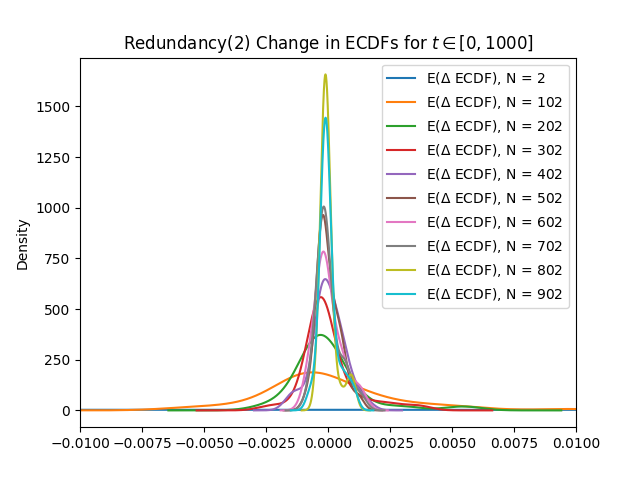
\includegraphics[width=0.7\linewidth]{redundancyecdf}
    \caption{Redundancy(2) ECDFs for Varying $N$}
    \label{fig:redecdf}
\end{figure}

\begin{figure}
    \centering
    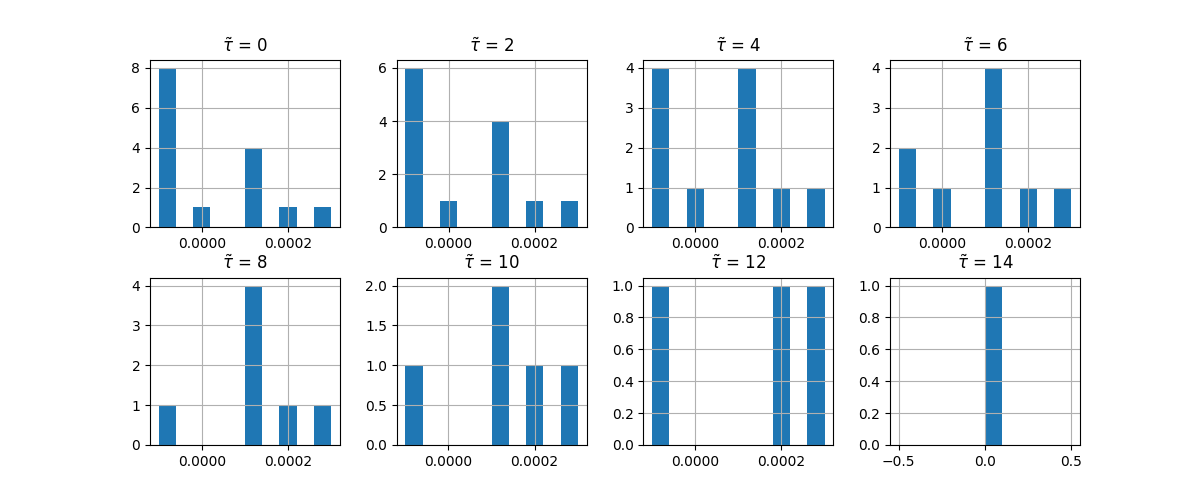
\includegraphics[width=0.8\linewidth]{redtau}
    \caption{Redundancy(2) Histograms of ECDF Changes for Varying $\tilde \tau$ at $N=1000$}
    \label{fig:taus}
\end{figure}

